\documentclass{report}
\usepackage[english]{babel}
\usepackage{microtype}
\usepackage{amsmath,amssymb}
\usepackage{amsthm}
\usepackage[round, authoryear]{natbib}
\usepackage[all]{xy}
\usepackage{array}
\usepackage{graphicx}
\usepackage{framed}
\usepackage{enumerate}
\usepackage{qtree}
\usepackage{mdframed}
\usepackage{tikz}
\usepackage{tikz-dependency}
\usepackage{algorithmic}
\usepackage{algorithm}
\usepackage{float}
\usepackage[OT2,T1]{fontenc}
\newcommand\textcyr[1]{{\fontencoding{OT2}\fontfamily{wncyr}\selectfont #1}}
\newcommand{\myparagraph}[1]{\paragraph{#1}\mbox{}\\}
\bibliographystyle{plainnat}
\renewcommand\topfraction{0.85}
\renewcommand\bottomfraction{0.85}
\renewcommand\textfraction{0.1}
\renewcommand\floatpagefraction{0.85}
\author{}
\title{}

%Define theorem style for definition and metric
\newtheoremstyle{break}  % follow `plain` defaults but change HEADSPACE.
  {\topsep}   % ABOVESPACE
  {15pt}   % BELOWSPACE
  {\itshape}  % BODYFONT
  {0pt}       % INDENT (empty value is the same as 0pt)
  {\bfseries} % HEADFONT
  {.}         % HEADPUNCT
  {\newline}  % HEADSPACE. `plain` default: {5pt plus 1pt minus 1pt}
  {}          % CUSTOM-HEAD-SPEC

\theoremstyle{break}
\newtheorem{metric}{Metric}
\newtheorem{notion}{Notion}
\newtheorem{definition}{Definition}
\def\citepos#1{\citeauthor{#1}'s (\citeyear{#1})}

%Define new float environment for tables that is boxed
\floatstyle{boxed}
\newfloat{tab}{tbp}{lop}
\floatname{tab}{Table}


\begin{document}
\tableofcontents

\chapter[3]{Empirical Research on Transfer Models}

%write a good introduction!!!!!
In the previous chapter we saw that almost all current state of the art models search for bijective mappings between tree structures of source and target sentences (such that parsing with an SCFG is possible). Blabla explain requirements


wat zijn de vragen:
- what does it mean for two sentences to have a compositional translation?
- how do we choose from all the available compositional structures
- how do we 
 both the target language and the source language

In the previous chapter was concluded that although almost all current state of the art MT models search for bijective mappings between tree structures of source and target sentences, it is still not 

Almost all current state of the art models search for bijective mappings between tree structures of source and target sentences, this is the subset wer are interested in (modelled by SCFG). For such a system to be perfect, it is required that both the source and target languages involved, as well as the translation, are perfectly compositional (anders). The extent to which this condition is true is not well understood, which raises the question: assuming language is at least to a certain extent compositional, how exploitable is this compositionality in translation. Complicated question, several subquestions
 In this chapter, we argue that such a complicated question should be addressed on an empirical level, and lay the groundwork for such an analysis. We will start by 

\begin{figure}[!ht]
\begin{framed}
\centering
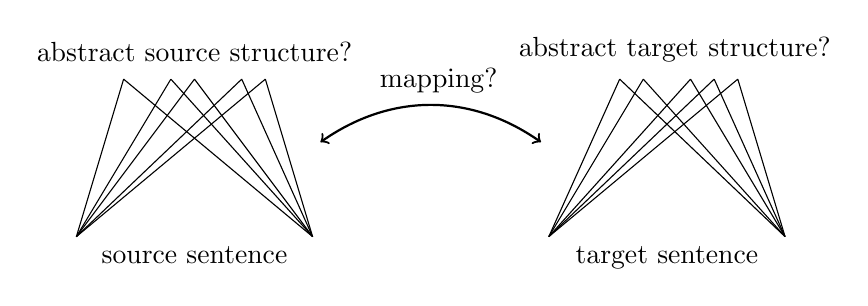
\begin{tikzpicture}

\coordinate (ss) at (1.5,0);
\node [below] at (ss) {source sentence};

%\draw[] (0,0) -- node[below]{source sentence} (3,0);
\draw (0,0) -- (0.6,2) (3,0) -- (0.6,2);
%\draw (0,0) -- (0.9,2) (3,0) -- (0.9,2);
\draw (0,0) -- (1.2,2) (3,0) -- (1.2,2);
\draw (0,0) -- (1.5,2) (3,0) -- (1.5,2);
%\draw (0,0) -- (1.8,2) (3,0) -- (1.8,2);
\draw (0,0) -- (2.1,2) (3,0) -- (2.1,2);
\draw (0,0) -- (2.4,2) (3,0) -- (2.4,2);

\node [above] at (1.5,2.1) {abstract source structure?};
\node [above] at (4.6,1.7) {mapping?};
\node [above] at (7.6,2.1) {abstract target structure?};
\coordinate (ts) at (7.5,0);
\node [below] at (ts) {target sentence};

%\draw (6,0) -- (0.6,2) (9,0) -- (6.6,2);
\draw (6,0) -- (6.9,2) (9,0) -- (6.9,2);
\draw (6,0) -- (7.2,2) (9,0) -- (7.2,2);
%\draw (6,0) -- (7.5,2) (9,0) -- (7.5,2);
\draw (6,0) -- (7.8,2) (9,0) -- (7.8,2);
\draw (6,0) -- (8.1,2) (9,0) -- (8.1,2);
\draw (6,0) -- (8.4,2) (9,0) -- (8.4,2);

\coordinate (startarrow) at (3.1,1.2);
\coordinate (endarrow) at (5.9,1.2);

\draw[<->,bend left =35, thick] (startarrow) to (endarrow);

\end{tikzpicture}
\end{framed}
\caption{Compositional translation}\label{fig:comptrans2}
\end{figure}



\section{Assumptions underpinning Transfer models}
\label{sec:assumptions}

%Section introduction
Compositionality of both language and translation are well discussed in the literature. In this section,


\subsection{Compositionality of Natural Language}

A language can be said to be compositional, if the set of expressions in it satisfy the following principle:

\begin{quote}
\textbf{The Principle of Compositionality}\\
The meaning of an expression is a function of the meaning of its parts and the syntactic rule by which they are combined \citep{partee1984compositionality}
\end{quote}

The principle applies rather obviously to (most) artificial languages. The meaning of their expressions can be unambiguously determined by considering the atoms and the rules used to combine them. For instance, consider the expression $p\lor q$ in propositional logic. Its truth-value can be determined by plugging in the truth values of $p$ and $q$ into the rule of the $\lor$-connective. Also programming languages can be interpreted by considering their basic units and the rules used to combine them.

Intuitively, it seems very reasonable that natural languages should obey this principle as well: we do not store the meaning of all possible sentences of language in our head, and we have no trouble understanding new sentences. Given that we can all perceive a certain systematicity and recursion in the way sentences are constructed (often referred to with the term `syntax'), the stand that we can derive the meaning of a new sentence by using some kind of rule to combine the meanings of the words in the sentence seems plausible.\footnote{There is no consensus in linguistics as to the cognitive reality of such a system. On the one hand, there is the Chomskian group of researchers, that advocate the existence of an underlying compositional grammar universal to all human beings \citep[As first claimed in][]{chomsky1956three}, while others believe no such system exist, and language users rely on some sense of familiarity with what they have heard before \citep[e.g.,][]{scha1990taaltheorie}. However interesting, we will not scrutinize this debate in this thesis, as we are interested in the observable compositionality of language, rather than how this is solved in our brains.} However, when trying to design a compositional grammar for language, it turns out that there are many obstacles, that can be summarised in following two, not unrelated, issues.(anders)

First of all, creating a grammar that covers \textit{all} grammatical utterances of a natural language, without generating too many ungrammatical ones, has proven a far from trivial task. Even for a finite (but reasonably sized) non-trivial corpus, it is surprisingly difficult to construct such a compositional grammar \citep{scha1990taaltheorie}. The bigger the grammar grows, the more phenomena need to be taken into account, as well as how they interact with each other. A glaring problem with this are idiomatic expressions (anders), whose meaning cannot be derived from its parts, that should be included as basic units, but can sometimes follow the basic rules as well (give example).

The second difficulty concerns ambiguity. In programming languages and logical languages, utterances typically have only one analysis, and their meaning is thus unambiguous.\footnote{Although ... give example and and and} Under all current existing grammar formalisms assigning structures to natural language, all sentences (of some length) have many different structural analyses, of which usually only one or two are perceived by humans \citep{scha1990taaltheorie}. Even sentences that are considered unambiguous by humans thus need to be disambiguated.\footnote{Note that this problem differs from one of the standard counter arguments of compositionality, that concerns sentences like `two men carry two chairs', that \textit{are} considered ambiguous by humans, but cannot be assigned two distinct syntactic analyses capturing this difference \citep{pelletier1994principle}. Not particularly relevant, but certainly nice to notice, is that this type of ambiguity is not necessarily problematic for translation, as it might be preserved. For instance, the Dutch translation `twee mannen dragen twee stoelen' of aforementioned sentence has the same two meanings as the English one.} In practice, when working with compositional grammars, this issue is often solved by assigning probabilities to the grammar rules, and computing the structure with the maximum probability (or an approximation of this).

%Maybe nog iets over janssen, en dat veel problemen wel een oplossing lijken te kennen
In conclusion, there are several problems that need to be solved when constructing a compositional grammar for language. Much is possible if the size of the atomic building blocks is taken to be flexible --> but then still compositional?
Blabla choices about syntactic rules and the size of the building blocks. blabla ,where the daunting question is: how much `extra' do we need if we have the meanings of the lexical items and the syntactic structure, what does this extra consist of anders). this is one of the problems.... we will get back to this later, after compositionality of translation

\subsection{Compositionality of Translation}

Compositionality of translation can be described with a principle analogue to the principle we saw for the compositionality of language:

\begin{quote}
\textbf{The Principle of Compositionality of Translation}\\
Two expressions are each others translation if they are built up from parts which are each other's translation, by means of translation-equivalent rules. (ref) \end{quote}

In other words, compositional translation takes place by identifying the compositional structure of the target language, mapping the syntactic rules to translation equivalent rules on the source side, and recursively determining the translation equivalence of the parts. Compositional translation is a very common method in translation between artificial languages \citep{janssen1996compositionality,janssen1998algebraic}. The translation from one logical language into another, or the translation the compiler performs when interpreting a programming language are all compositional. When considering a purely semantical compositional grammar, it seems that compositionality of translation should also hold for natural language, but there are several issues that complicate compositional translation of natural language.
First of all, an assumption prevalent in the principle, is that in translation not only meaning, but also form should be preserved (as much as possible). In other words, it assumes that translation is literal. For artificial languages this property is straight-forward and useful, mostly because there are no a priori reasons to prefer a non-literal translation over a literal translation. In natural language, this assumption is rather questionable. There are many occasions in natural language in which the assumption seems fairly applicable. It captures, for instance, the fact that `all ravens are black' is an adequate translation of `alle raven zijn zwart', while the logically equivalent `if something is not black, it is not a raven' is not \citep{landsbergen1989power}. However, in practice a translator can have many reasons to prefer a free translation, even if a more literal alternative is also available. For the moment, we will try to ignore this issue. Given the current state of MT, that is not (yet) focussing on literary translations, it seems acceptable to prefer a correct literal translation, even if this stylistically would not have been the first choice of human translator.

Even when regarding the most literal translation the best one, translation is not always literal, which brings us to the problem of syntactic and lexical translational divergences. Languages doe not always express the same set of meanings, or express meanings in the same way. Even in languages of cultures that are quite similar, one can find a number of words that simply do not have an adequate translation in the other language (e.g., in translation between English and Dutch the words `gezellig' and `evidence' do not seem to have a clear equivalent in the other language), and even if the same meaning is expressed there are many syntactic phenomena in natural language that seem to be problematic for a compositional translation. For example: different ways of role expression (e.g., `I like (obj)' and `\textcyr{mne nravitsa (subj)}') or syntactic mismatches (e.g., `woonachtig zijn' and its translation `reside' \citep{landsbergen1989power}).  The grammar rules and basic units can thus not simply be taken from a monolingual grammar, as there is no guarantee that the rules and basic units will have a translation equivalent rule or basic unit in the other grammar. The grammars must be constructed for translation, such that they are `attuned' \citep{rosetta1994compositional}. \cite{rosetta1994compositional} showed that previous mentioned examples do not necessarily stand in the way of compositional translation, by manually constructing a grammar for translation from English to Dutch, covering many non-trivial translation phenomena. However, their grammar consist of separate semantic and syntactic formalisms, which makes their case more complicated than the more direct structure mapping we are interested in for this thesis.

In conclusion .... say which problems we need to solve, and that we once again do not know how compositional our system is after we have solved our problems.

\subsection{Compositionality of Language and Translation}

Not yet sure what I want to say here, and whether I need this subsection at all.

\section{Representations of Compositionality}

Our ultimate goal is to measure the compositionality of actual data, blabla thus we need to have a method to identify it... 

Introduction that makes clear that we must be able to identify and represent compositionality, maybe here I somehow need to get to the corpora, in which compositionality is not discernible.

To be able to investigate compositionality of both language and translation on an empirical level, we need to be able to identify compositionality when we see it. In this section, we will explain how compositionality manifests itself in practice and how a compositional structure can be represented. This section is very basic, but also very important, and will therefore be treated nevertheless.

\subsection{Compositional Representations of Language}

%Ik weet nog niet helemaal hoe ik dit nu goed moet doen, later nog naar kijken
A compositional representation of a sentence should recursively describe how it was built up from its parts, which can be described in a tree structure

A compositional structure of a sentence, describes how it was constructed from its parts, which can be captured in a tree structure. We will explain this using an example. Consider the simple sentence `I gave my little brother a new toy car.'. There are very many ways, in which this sentence could be built up from its parts, such as:\begin{itemize}
\item Use rule A to combine `brother' and `a' to get `brother a'
\item Use rule B to combine `I', `gave', `my' and `little' to get `I gave my little'
\item Use rule C to combine `new', `toy' and `car' into `new toy car'
\item use rule D to combine `I gave my little' and `brother a' to get `I gave my little brother a'
\item Use rule E to combine `I gave my little brother a' and `new toy car' to get the entire sentence
\end{itemize}

This construction can be represented in a tree structure (\ref{fig:struct1}), that describes which parts were combined in the application of one syntactic rule. 

\begin{figure}[!ht]
\centering
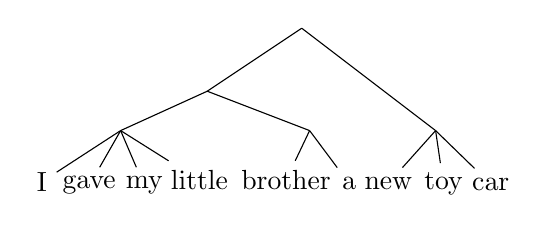
\begin{tikzpicture}
\node (I) at (1,0.05) {I};
\node (gave) at (1.6,0) {gave};
\node (my) at (2.3,0) {my};
\node (little) at (3.0,0.07) {little};
\node (brother) at (4.1,.07) {brother};
\node (a) at (4.9,0.03) {a};
\node (new) at (5.4,0.03) {new};
\node (toy) at (6.1,0.02) {toy};
\node (car) at (6.7,0.02) {car};

\coordinate (Igavemylittle) at (2,0.7);
\coordinate (brothera) at (4.4,0.7);
\coordinate(newtoycar) at (6.0,0.7);
\coordinate (all) at (4.3,2);
\coordinate (Igavemybrothera) at (3.1, 1.2);

\foreach \from/\to in {Igavemylittle/I, Igavemylittle/gave, Igavemylittle/my, Igavemylittle/little, a/brothera, brother/brothera, newtoycar/new, newtoycar/toy, newtoycar/car, Igavemybrothera/Igavemylittle, Igavemybrothera/brothera, all/newtoycar, all/Igavemybrothera}
	\draw (\from) -- (\to);

\end{tikzpicture}
\caption{A tree that describe how the sentence 'I gave my little brother a new toy car' could have been compositionally constructed.}\label{fig:struct1}
\end{figure}

Formally, there is no reason to discard the tree structure from Figure \ref{fig:struct1}, yet everyone that understands the English language will agree that this structure makes syntactically little sense, as we perceive that other parts somehow belong together, such as `my little brother', or `a new toy car'. The structures in Figure \ref{fig:struct2} therefore seem more plausible.

\begin{figure}[!ht]
\centering
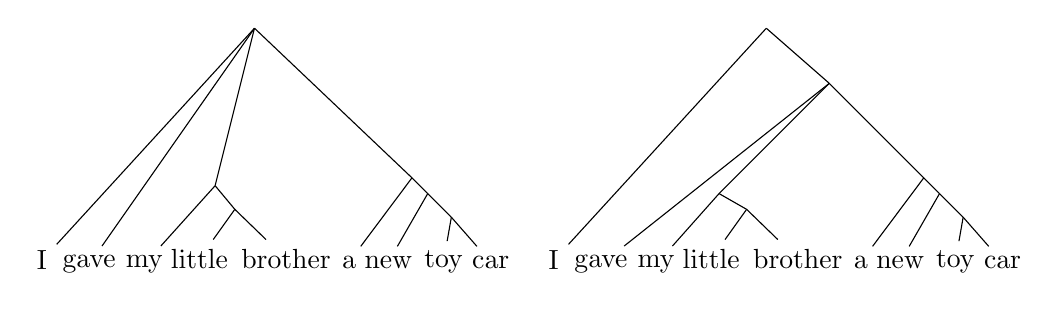
\begin{tikzpicture}

\node (I) at (0,0.05) {I};
\node (gave) at (0.6,0) {gave};
\node (my) at (1.3,0) {my};
\node (little) at (2.0,0.07) {little};
\node (brother) at (3.1,.07) {brother};
\node (a) at (3.9,0.03) {a};
\node (new) at (4.4,0.03) {new};
\node (toy) at (5.1,0.03) {toy};
\node (car) at (5.7,0.03) {car};

\coordinate (toycar) at (5.2,0.6);
\coordinate(newtoycar) at (4.9,0.9);
\coordinate (anewtoycar) at (4.7,1.1);
\coordinate (littlebrother) at (2.45,0.7);
\coordinate (mylittlebrother) at (2.2,1);
\coordinate (all) at (2.7,3);

\foreach \from/\to in {toycar/car, toycar/toy, newtoycar/toycar, newtoycar/new, anewtoycar/newtoycar, anewtoycar/a, littlebrother/brother, littlebrother/little, mylittlebrother/littlebrother, mylittlebrother/my, all/I, all/gave, all/mylittlebrother, all/anewtoycar}
	\draw (\from) -- (\to);

\node (I_) at (6.5,0.05) {I};
\node (gave_) at (7.1,0) {gave};
\node (my_) at (7.8,0) {my};
\node (little_) at (8.5,0.07) {little};
\node (brother_) at (9.6,.07) {brother};
\node (a_) at (10.4,0.03) {a};
\node (new_) at (10.9,0.03) {new};
\node (toy_) at (11.6,0.03) {toy};
\node (car_) at (12.2,0.03) {car};

\coordinate (toycar_) at (11.7,0.6);
\coordinate(newtoycar_) at (11.4,0.9);
\coordinate (anewtoycar_) at (11.2,1.1);
\coordinate (littlebrother_) at (8.95,0.7);
\coordinate (mylittlebrother_) at (8.6,0.9);
\coordinate (gavetobrother_) at (8.1,1.3);
\coordinate (gavetocar_) at (10,2.3);
\coordinate (all_) at (9.2,3);

\foreach \from/\to in {toycar_/car_, toycar_/toy_, newtoycar_/toycar_, newtoycar_/new_, anewtoycar_/newtoycar_, anewtoycar_/a_, littlebrother_/brother_, littlebrother_/little_, mylittlebrother_/littlebrother_, mylittlebrother_/my_, all_/I_, gavetocar_/gave_, gavetocar_/mylittlebrother_, gavetocar_/anewtoycar_, all_/gavetocar_}
	\draw (\from) -- (\to);
\end{tikzpicture}
\caption{Possible compositional structures for the sentence `I gave my little brother a new toy car'}\label{fig:struct2}
\end{figure}

Such tree representations can be used to capture any compositional structure: every node corresponds to the application of a syntactic rule in the derivations, where its children were the arguments. Some compositional structures, however, cannot be represented by tree structures as simple as the ones we just saw. Consider for instance the case in which one of the parts used in the translation was non-contiguous. It is very common to assume that the nodes in the tree (corresponding to the parts) constitute contiguous sequences in the sentence, as such structures can be generated by context-free grammars. Sometimes, this gets in the way, as can be concluded from the example depicted in Figure \ref{fig:struct3}, where the parts that naturally belong together are found in different places of the sentence.\footnote{Note that this structure is mathematically still a tree, of which the branches cross due to the fact that the leafs of the tree are not linearly ordered.}

\begin{figure}[!ht]
\centering
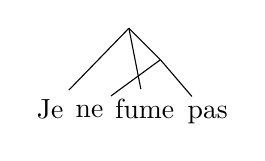
\begin{tikzpicture}

\node (je) at (0,0.07) {Je};
\node (ne) at (0.5,0.04) {ne};
\node (fume) at (1.2,0.08) {fume};
\node (pas) at (2,0) {pas};

\coordinate (nepas) at (1.4,0.7);
\coordinate (jefume) at (0.6,0.7);
\coordinate (all) at (1.0,1.1);

\draw (nepas) -- (ne);
\draw (nepas) -- (pas);
\draw (je) -- (all);
\draw (fume) -- (all);
\draw (all) -- (nepas);

\end{tikzpicture}
\caption{'non-projective' tree}\label{fig:struct3}
\end{figure}


finishing statement

\subsection{Representations of compositional Translations}

%deze subsectie moet duidelijk helemaal herschreven worden, maar ik weet nog niet zo goed hoe..
Representations of compositional translations are representation-wise very similar to compositional structures of language: they are tree representations that describe how the sentence was compositionally translated. The main difference between the two types of structures (besides what they are describing, of course), lies in the notion of parts. In compositional language structures the parts were sequences of words that were combined through syntactic relations, while in compositional translation structures, the parts are defined through translation equivalence. Consider, for instance, picture describing a possible translation for the sentence pair (I give my little brother a ball, Ik geef mijn kleine broertje een bal), in which the translation equivalence is made explicit through linking the  `parts' that were used in the translation. Note that if tree pairs are constructed as such through compositionality, every source node tree has an equivalent target node tree, the two resulting trees are thus isomorphic. %dit heb ik eigenlijk al eerder gezegd volgens mij, miss moet ik dit hier anders brengen, als een soort van `after bewijs'

\begin{figure}[!ht]
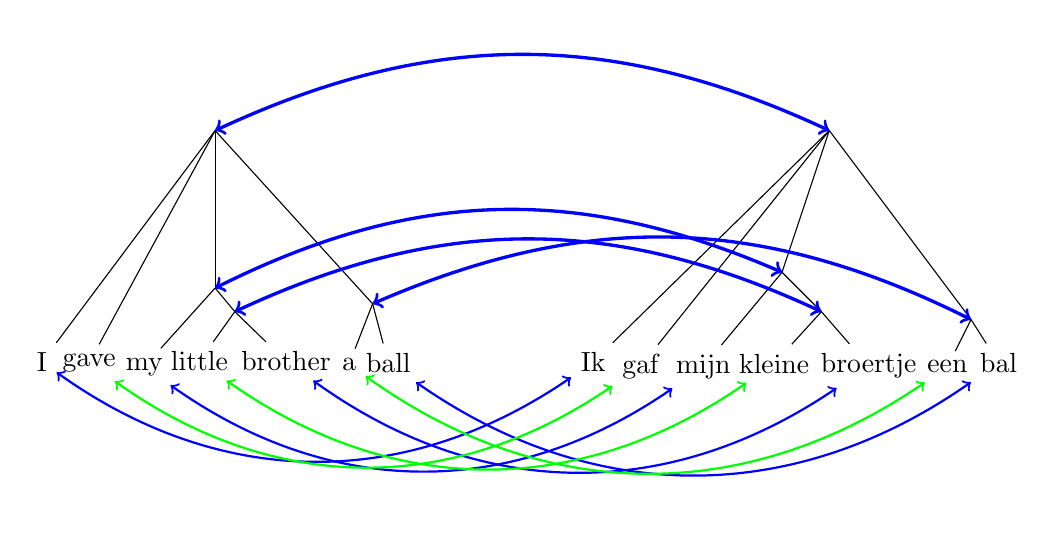
\begin{tikzpicture}
\node (I) at (1,0.06) {I};
\node (give) at (1.6,0.05) {gave};
\node (my) at (2.3,0) {my};
\node (little) at (3.0,0.07) {little};
\node (brother) at (4.1,0.07) {brother};
\node (a) at (4.9,0.03) {a};
\node (ball) at (5.4,0.05) {ball};

\coordinate (toycar) at (5.6,0.7);
\coordinate (littlebrother) at (3.45,0.7);
\coordinate (mylittlebrother) at (3.2,1);
\coordinate (aball) at (5.2,0.8);
\coordinate (all) at (3.2,3);

\foreach \from/\to in {aball/ball, aball/a, littlebrother/little, littlebrother/brother, mylittlebrother/my, mylittlebrother/littlebrother, all/give, all/mylittlebrother, all/aball, all/I}
	\draw (\from) -- (\to);
	
\node (Ik) at (8,0.06) {Ik};
\node (geef) at (8.6,0) {gaf};
\node (mijn) at (9.4,0) {mijn};
\node (kleine) at (10.3,0.04) {kleine};
\node (broertje) at (11.5,0.01) {broertje};
\node (een) at (12.5,0) {een};
\node (auto) at (13.15,0.05) {bal};

\coordinate (kleinebroertje) at (10.9,0.7) {};
\coordinate (mijnkleinebroertje) at (10.4,1.2);
\coordinate (eenauto) at (12.8,0.6);
\coordinate (alles) at (11,3);

\foreach \from/\to in {eenauto/auto, eenauto/een, kleinebroertje/kleine, kleinebroertje/broertje, mijnkleinebroertje/mijn, mijnkleinebroertje/kleinebroertje, alles/Ik, alles/geef, alles/mijnkleinebroertje, alles/eenauto}
	\draw (\from) -- (\to);	

\foreach \from/\to in {all/alles, mylittlebrother/mijnkleinebroertje, littlebrother/kleinebroertje, aball/eenauto}
	\draw[<->, bend left =25, very thick,blue] (\from) to (\to);

\foreach \from/\to in { broertje/brother,  mijn/my, Ik/I, auto/ball}
	\draw[<->, bend left =35, thick,blue] (\from) to (\to);

\foreach \from/\to in {een/a,  kleine/little, geef/give}
	\draw[<->, bend left =35, thick,green] (\from) to (\to);

\end{tikzpicture}

\caption{linked structures}\label{fig:transtrees}
\end{figure}

Unfortunately, the complexity of the given example is far below average. The example shows no translational divergence complicating the establishment of translation equivalence, the sentences have the same length, no reordering takes place, and all translation equivalent sequences are contiguous. In fact, the target sentence is a word for word translation of the source sentence, which means that any source structure could be mapped to an isomorphic target structure through translation equivalence.

To establish isomorphism in harder cases, a phrasal approach is required. In Figure \ref{fig:phrasal}, a very simple example is given, of the translation of the three word phrase `a toy car' into the two word phrase `een speelgoedautootje'.

\begin{figure}[!ht]
\centering
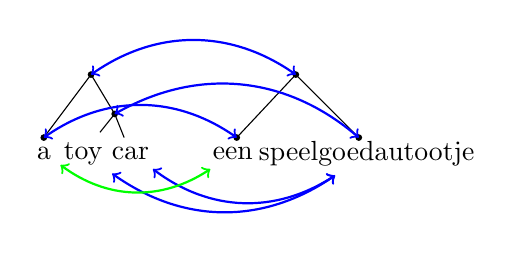
\begin{tikzpicture}

\node (a) at (0,0) {a};
\node (toy) at (0.5,0) {toy};
\node (car) at (1.1,0) {car};
\node (een) at (2.4,0) {een};
\node (auto) at (4.1,0) {speelgoedautootje};

\filldraw (0,0.2) circle (0.035);
\filldraw (2.45,0.2) circle (0.035);
\filldraw (4.0,0.2) circle (0.035);
\filldraw (0.9,0.5) circle (0.035);
\filldraw (0.6,1) circle (0.035);
\filldraw (3.2,1) circle (0.035);

\coordinate (toycar) at (0.9,0.5);
\coordinate (a_) at (0,0.2);
\coordinate (een_) at (2.45,0.2);
\coordinate (auto_) at (4.0,0.2);
\coordinate (all) at (0.6,1);
\coordinate (allnl) at (3.2,1);

\foreach \from/\to in {toycar/toy, toycar/car,all/toycar, all/a_, allnl/een_, allnl/auto_}
	\draw (\from) -- (\to);	

\foreach \from/\to in {auto/car,  auto/toy, a_/een_, toycar/auto_, all/allnl}
	\draw[<->, bend left =35, thick,blue] (\from) to (\to);

\draw[<->, bend left = 35, thick, green] (een) to (a);

\end{tikzpicture}
\caption{Phrasal translation equivalence}\label{fig:phrasal}
\end{figure}

From the previous two examples, it is not yet clear how such translation structures deal with reordering. It is important to realise that translation equivalence of two phrases does not imply that the order \textit{within} the phrases is identical. The phrases `una casa comoda' and `een comfortabel huis' are translation equivalent, even though the noun adjective order is not the same. Reordering by permuting the children in a parse tree is in practice quite powerful, although theoretically the fraction of reorderings that can be accounted for rapidly decreases with the length of the sentence \citep{satta2005some}.

Note that reordering amplifies the need of rules. Without them, it is impossible to always correctly guess the order of the leaf nodes of the target side tree.





\subsection{Compositionality of both in practice?}



%%%%%%%%%%%%%%%%%%%%%%%%%%%%%%%%%%%%%%%%%%%%%%%%%%%%%%%%%%%%
%CONCRETE SYSTEMS FOR COMPOSITIONALITY
%

\section{Concrete systems for Compositionality}

Thus far, we have discussed compositional translation on a practical but yet unspecific level, as we have relied on intuitition to determine both linguistic and translation equivalence parts (and the structures emerging from them). To analyse compositionality of large corpora with translation data, mechanisms to establish compositional structures and translation equivalence automatically and on a large scale are required. In this section, we will discuss a method for determining a compositional structure for language (nu al motiveren waarom maar een?)
 these methods, which will be the last step before putting everything into place for real empirical research of compositionality (anders).

\subsection{Monolingual Compositionality: Dependency Structures}

There are many monolingual grammar formalisms, few of which have parsers that can efficiently assign structures to large corpora of text. The most common formalisms in MT are finite state machines, constituent grammars, and dependency grammars. Although some cognitive researchers might disagree about the workings in the mind \citep[e.g.]{frank2012hierarchical}, the expressibility of finite state machines is generally considered to week to account for the complex phenomena occurring in natural language, and we will therefore disregard them for the rest of this thesis.

Constituency grammars have shown to be a quite suitable model for natural language, although natural language does not seem to be entirely context free \citep{shieber1987evidence}. As described in Section (ref???), different researchers have already tried to incorporate syntactic information from constituency grammars in translation models, but they are hindered by the fact that constituency grammars give a purely syntactic analysis of a sentence, and constituents are often not preserved during translation, which we will further discuss in section ref???.

In this thesis, we will therefore focus on the third option: dependency grammars. Dependency parses have been shown to stay better preserved during translation than constituency grammars \citep{fox2002phrasal}, and given their semantic motivation, dependency grammars seem very suitable for the task at hand. We will shortly discuss the motivation and background of dependency grammars, give a formal definition, and provide some clarifying examples.

\subsubsection{Background}

Contrary to phrase structure grammars, that establish relations between constituents of a sentence, a dependency grammar does not divide sentences in phrases. Rather, it is based on the idea that in a sentence all words but one depend on another word in the sentence, via a(n asymmetric) binary relationship that describes how the former word modifies or complements the latter. For instance, in the sentence `I really like writing my thesis', `my' depends on `thesis', as it complements it, and `really' depends on `like', which it modifies. Words can be said to have a valency, depending on how many dependents they need to be saturated (e.g., `like' would have a valency of two 2, as it needs both a subject and an object).

Although traditional dependency grammar (DG) has been used by linguists since the Middle Ages \citep{covington1990dependency}, modern DG is often seen as being created by \cite{tesniere1959elements}, whose cognitive motivation for it is worth citing:

\begin{quote}
The sentence is an organised whole; its constituent parts are the words. Every word that functions as part of a sentence is no longer isolated as in the dictionary: the mind perceives connections between the word and its neighbours; the totality of these connections forms the scaffolding of the sentence. The structural connections establish relations of dependency among the words. Each such connection in principle links a superior term and an inferior term. The superior term receives the name governor; the inferior term receives the name dependent. \citep[Translation:][]{ryan2013}
\end{quote}

The criteria for being a head-dependent pair are a mix of syntactic and semantic criteria \citep{nivre2005dependency}, and generally depend on the grammatical function the sentence or with respect to the word it depends on. Not all dependency grammars are identical in the relations they are considering, and their treatment of certain intuitively problematic constructions as coordination and conjunction \citep{nivre2005dependency}. In this thesis, we will follow the convention used in \cite{de2006generating}.

\subsubsection{Formally}

A dependency grammar is formally defined as follows \citep{hays1964dependency,gaifman1965dependency}:

\begin{definition}[Dependency Grammar]\label{def:depgram}
A dependency grammar is a quadruple $\langle R,L,C,F\rangle$, consisting of a set $L$ of terminal symbols (lexemes), a set $C$ of auxiliary symbols (lexical categories), a $R$ set of dependency rules over the auxiliary symbols $C$, and an assignment function $F : L\rightarrow C$.
\end{definition}

An example of a very simple (and unplausible) dependency grammar (according to which the dependency parse in Figure \ref{fig:depgraph} is grammatical) is shown in Figure \ref{fig:depgrammar}.

\begin{figure}[!ht]
\begin{framed}
$\mathcal{D} = \langle R,L,C,F\rangle$, where:\begin{enumerate}
\item[] $L$ = \{My, dog, also, likes, eating, sausage\}
\item[] $C$ = \{poss, nsubj, xvmod, xcomp, dobj, root\}
\item[] $R$ = \{(root, nsubj), (nsubj, poss), (root, xcomp), (xcomp, dobj), (root, xvmod)\}
\item[] $F = \left\{
  \begin{array}{l l l}
	F\text{(My)=poss} & \quad F\text{(dog)=nsubj} & \quad F(\text{(also)=xvmod}\\
	F\text{(likes)=root}& \quad F\text{(eating)=xcomp} & \quad F\text{(sausage)=dobj} 
  \end{array} \right.$
\end{enumerate}
\end{framed}
\caption{A Toy Dependency Grammar}\label{fig:depgrammar}
\end{figure}


\noindent A dependency grammar prescribes dependency structures of sentences, that can be interpreted as graphs that satisfies the criteria that it is rooted and has only a single head (in other words, a dependency structure is a tree):

\begin{definition}[Dependency Graph]\label{def:depgraph}
A dependency graph of a sentence $s = w_1~\ldots~w_n$ is a directed acyclic graph $\mathcal{G} = \langle V, E\rangle$, in which $V = \{w_1, \ldots,w_n\}$ and $E$ is a set of edges such that $(w_i,w_j)\in E$ if and only if there is a dependency relation between $w_i$ and $w_j$. Furthermore, the graphs satisfies the following two criteria:
\begin{enumerate}
\item $\exists\negthinspace w\in\negthinspace V$ s.t. $\forall w'\negthinspace\in\negthinspace V~(w,w')\negthinspace\notin\negthinspace E$ \hfill (rootedness)
\item $\forall w_1 w_2 w_3\negthinspace \in\negthinspace V\Big( (w_1,w_3)\negthinspace\in\negthinspace E~\land~(w_2,w_3)\negthinspace \in\negthinspace E\Big) \rightarrow w_1\negthinspace=\negthinspace w_2$ \hfill (single-headedness)
\end{enumerate}
The edges in $\mathcal{G}~$can be labeled with the function of the dependent.
\end{definition}

\noindent An example of a dependency graph is depicted in Figure \ref{fig:depgraph}. As the general definition of a graph is used, it is not immediately clear how  Definition \ref{def:depgraph} and Definition \ref{def:depgram} relate. To clarify: the set of vertices $V$ in $\mathcal{G}$ correspond to the lexical items, and thus with the set $L$ in a dependency grammar. The edges $V$ correspond to the dependency relations $R$, while their labels must be in $C$. The function $F$ describes which functions words are allowed to have in the sentence. 

\begin{figure}[!ht]
\centering
\begin{dependency}[theme=simple]%[hide label]
\begin{deptext}[column sep=.5cm, row sep=.1ex]
%PRP\$ \& NN \& RB \&[.5cm] VBZ \& VBG \& NN \\
My \& dog \& also \& likes \& eating \& sausage \\
\end{deptext}
\deproot{4}{}
\depedge{2}{1}{poss}
\depedge{4}{2}{nsubj}
\depedge{4}{3}{xvmod}
\depedge{4}{5}{xcomp}
\depedge{5}{6}{dobj}
\end{dependency}
\caption{Dummy Dependency Graph, find other later}\label{fig:depgraph}
\end{figure}

A condition often put on dependency graphs, is projectivity, that prescribes a linear ordering of the nodes in the tree. Projectivity simplifies parsing, as it reduces the search space, but it is often argued that it deprives dependency grammar from its most important asset \citep{covington1990dependency,debusmann2000introduction}: the elegant method for handling discontinuous constituents (see Figure \ref{fig:npdeptree}). For fixed word order languages like English, in which phrases belonging together tend to stay together, projectivity is thus a reasonable criterion, but to account for languages in which there are less restrictions on the word-order (e.g., Russian, Latin) non-projectivity is often required to provide an intuitive analysis. An example of a non-projective in a otherwise fixed word-order language (Dutch) is depicted in Figure \ref{fig:npdeptree}.

\begin{figure}[!ht]
\centering
\begin{dependency}[theme=simple]%[hide label]
\begin{deptext}[column sep=.5cm, row sep=.1ex]
Ik \& weet \& dat \& hij \& me \& liet \& winnen\\
\tiny{I} \& \tiny{know} \& \tiny{that} \& \tiny{he} \& \tiny{me} \& \tiny{let} \& \tiny{win}\\
\end{deptext}
\deproot{2}{}
\depedge{2}{1}{}
\depedge{2}{6}{}
\depedge{6}{3}{}
\depedge{6}{4}{}
\depedge{6}{7}{}
\depedge{7}{5}{}
\end{dependency}
\caption{Non projective dependency graph of the Dutch sentence `Ik weet dat hij me liet winnen'.}\label{fig:npdeptree}
\end{figure}

\subsection{Bilingual Compositionality: Alignment Trees}

Establishing translation equivalence on a large scale is often done by means of word-alignments (which we have briefly described when discussing the IBM models), which are mappings from source to target words that describe which target words were involved in the translation of which source words. An example is given in Figure \ref{fig:alignment}. Word-alignments give rise to a straight-forward notion of translation equivalence: two sequences of words are translation equivalent if the words in the one sequence are translated only into words in the other sequence, and vice versa (we will later put this on a more formal footage). The task of determining translation equivalence is herewith thus reduced to aligning sentences on a word-level. However also word-alignments are not directly discernible when looking at a sentence and translation, and thus need to be learned. In this section, we will discuss the most common method to learn word alignments. After giving the formal definition of a word-alignment we will briefly discuss the different types of word-alignments that exist (and how they influence translation equivalence) and how they can be obtained.

\begin{figure}[!ht]
\centering
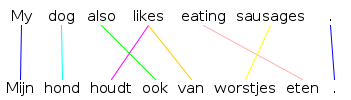
\includegraphics[scale=0.6]{alignment.png}
\caption{Word-alignments can be visualised in many ways. In this thesis, we will visualise alignments using lines, or arrows, where an arrow from source word $w_s$ to target word $w_t$ implies that $w_t$ was involved in the translation of $w_s$. The current figure shows a one-to-one alignment of the Dutch sentence `Na regen komt zonneschijn' and its translation `Auf regen folgt sonneschein'. The picture was generated by the alignment visualiser created by \cite{maillette2010visualizing}}
\label{fig:alignment}
\end{figure}

\subsubsection{Formal}

The precise definition of a word-alignment varies from paper to paper. Throughout this thesis we will use the following definition:

\begin{definition}[Alignment]\label{def:alignment}
Given a source sentence $s = s_0 \ldots s_n$ and its translation $t = t_0 \ldots t_m$, an alignment is a set $a \subseteq \{0,1,\ldots,n\} \times \{0,1,\ldots,m\}$ such that $(x,y)\in a$ iff $s_x$ is translated into $t_y$.
\end{definition}

In some definitions unaligned words are explicitly included in the alignment by adding an extra $NULL$ token to both source and target sets and including $(x,NULL)$ (or ($(NULL,y)$) in $a$ whenever word $x$ (or $y$) is unaligned. In our definition, unaligned words are not explicitly included: when a word $x$ is unaligned, this will be indicated by the absence of a word $y$ such that, respectively, $(x,y)$ or $(y,x)$, depending on whether $x$ was a source or target word. 


\subsubsection{Types of Word-alignments}

In the alignment in Figure \ref{fig:alignment}, every source word is aligned to exactly one target word and vice versa. Such an alignment is called a one-to-one alignment. It is also possible for source and target words to be aligned to more than one word, or to none at all, resulting in alignments that are one-to-many, many-to-one or even many-to-many. Another interesting property of the alignment depicted in Figure \ref{fig:alignment}, is that the target word order is identical to the source word order, resulting in an alignment in which none of the alignment links are crossing. Such an alignment is called monotone. The number of possible translation structures is largely determined by the complexity of the alignment, with rule of thumb: the simpler the alignment, the higher the number of possible structures. A summary of the restrictions corresponding to these different types of alignments is provided in Table \ref{table:alignments}.

\begin{table}[!ht]
\footnotesize{
\begin{tabular}{|ll|}
\hline
one-to-one & $\forall x\forall y \big( (x,y)\in y \to \forall z \big( (z,y)\in a \to z=x \land (x,z) \in a \to z=y \big ) \big ) $\\
&\\
one-to many & $\forall x\forall y \big( (x,y)\in y \to \forall z \big( (z,y)\in a \to z= x \big) \big) $\\
&\\
many-to-one & $\forall x\forall y \big( (x,y)\in y \to \forall z \big( (x,z)\in a \to z=y \big) \big ) $\\
&\\
many-to-many & - \\
&\\
monotone & $\forall w \forall x\forall y \forall z \big ( \left ( (x,y)\in a \land (w,z)\in a \land x < w \right ) \to y < z \big )$\\
\hline
\end{tabular}
}
\caption{Alignment types, restrictions}
\label{table:alignments}
\end{table}

\subsubsection{Translation Equivalence through Word-alignments}

Now that we have defined alignments, we can define translation equivalence. We will use the term `translation equivalent units' to refer to sequences that could have been `parts' in translation.

\begin{definition}[Translation Equivalence]
If $(s,t)$ is a pair of source and target sentences, and $A$ an alignment between $s$ and $t$. two sets of source and target words $w_s$ and $w_t$ are translation equivalent if and only if $$\forall x,y ( x\in w_s~(x,y)\in A \rightarrow y\in w_t \land x,y \in w_t~(y,x)\in A \rightarrow x\in A))$$
\end{definition}

The definition expresses the intuition that two sequences of words are translation equivalent, if the words in the first sequence are translated only into words in the second sequence, and vice versa. This definition does not includes a clause that states that such sequences need to be contiguous, a requirement that is often imposed in translation models as contiguous sequences are much easier to use in practice (and correspond to context freeness).

\subsubsection{Generating Word-alignments}

Even besides the fact that word-alignments are not visible in translation data, it is not always easy to establish which source words should be aligned to which target words. We will give two examples to illustrate this.

The first problematic cases are idiomatic expressions. The expression `Every cloud has a silver lining'  is synonymous with `Na regen komt zonneschijn', but it is unclear what would be a good alignment. Arguably, `has' should be aligned with `komt', as they are the only verbs in the sentence pair. However, when asking a bilingual Dutch and English speaker if `has' is a proper translation of `komt', the odds of obtaining a affirmative answer would be very slim. A more plausible alignment would align every Dutch word to every English words, indicated that the expression is translated as a whole. Such an alignment is called a phrasal alignment.

Problems also arise in the translation of function words, that do not have a clear translation equivalent in the other language. Consider, for instance, the word `does' in the sentence pair `John does not live here, John wohnt hier nicht'. As `does' has no clear translation in German, one might argue that it should be unaligned. However, the word seems to be connected with `live', so it could also be aligned with `wohnt'. A third option is to align `does' to `nicht', as it appeared with `not' when the sentence was negated.\citep[Example from][p.114]{koehn2008statistical}

\myparagraph{Manual Word-alignments}
In manually aligned corpora, the issues raised in the previous paragraph are often addressed by distinguishing sure alignment links and possible alignment links \citep{lambert2005guidelines}. The sure alignment links (indicated by the letter S) then represent unambiguous alignment links, while the possible alignment links (P) are less certain. Possible alignment links appear in case of phrasal translations, ambiguous translations, or in case two annotators disagree. 

There are very few manually aligned corpora, the only ones known to the author are presented in \cite{och2000improved}, \cite{graca2008building}, \cite{mihalcea2003evaluation} and \cite{pado2006optimal}, \cite{ahrenberg2000evaluation}. Short description of these corpora??
Manually annotating translation corpora is very labour intensive and none of these corpora are big enough to train models on. Rather, they are used to evaluate automatically generated word-alignments. A common metric used for this task is the alignment error rate (AER), that is defined as follows (ref?):

$$
\text{AER(S;P;A) = } - \frac{|\text{A}\cap\text{S}| + |\text{A}\cap\text{P}|}{|\text{A}| + |\text{S}|}
$$

A perfect score can thus be achieved by an alignment that has all the sure alignment points and some of the possible alignment points.

\myparagraph{Automatic Word-alignments}
Word alignments are established as a by-product for the word-based IBM models, and despite multiple efforts to improve on these alignments (e.g., refs), it is still common practice to use the alignments produced by the SMT toolkit used to train the IBM models \citep{och03:asc}. We will not discuss further methods for automatically word aligning corpora, but just briefly explain how the IBM alignments arise, and how many-to-many alignments are derived from them.

One step in the IBM models, is to learn a lexical translation model from a parallel corpus. If a word-alignment was directly visible from the data, this would be an easy task, as one could just count for each word how often it occurred in the text and how it was translated, and estimate a probability from these counts using relative frequency estimation (which happens to be the maximum likelihood solution) (anders). Conversely, given the lexical probability model, the most possible word-alignment could be estimated. Learning word-alignments and lexical probabilities from a parallel corpus can thus be seen as a problem of incomplete data, that can be addressed with the expectation maximization (EM) algorithm \citep{dempster1977maximum}, which works as follows:\begin{enumerate}
\item Initialize the lexical probabilities (often with uniform distributions).
\item Compute the most probable alignment from the lexical probabilities (expectation).
\item Recompute the lexical probabilities from the alignment found in the previous step (maximization)
\item Iterate steps 2 and 3 until convergence.
\end{enumerate}

\noindent Note that the use of such an algorithms means that the larger the corpus, the better the resulting alignments. It is thus not possible to align just one sentence.

In IBM model 1 and 2, the models that describe how the alignments depend on the lexical probabilities are sufficiently simple to exhaustively run the EM algorithm, and a (global) optimum is thus guaranteed to be found. To find the most probable alignments in the higher IBM models, stochastic hill climbing is used. Excellent examples of how the algorithm works on the IBM models can be found in \cite[p88-113]{koehn2008statistical}.

%Check order
The IBM models consider the sequence of target words as being generated by the source words one by one. Therefore, although source words can be aligned to more target words, every target word is aligned to at most one source word and the resulting alignments are thus many-to-one. However, many-to-many alignments are often desired, as they are very common in practice. Alignments used to train SMT models on are often created by running the IBM models in both directions, and combining the resulting alignments. The three most common methods of merging two alignments $A_1$ and $A_2$ are:\begin{enumerate}
\item Union: $A_1\cup A_2$, containing all links from both alignments. The recall of the union will be high (as it contains many links), but as it contains all faulty alignment links from both alignments too, the precision is often quite low.\footnote{Given a set of desired alignment points $A_{gold}$, recall and precision of an alignment $A$ are defined as follows:\\
$$\text{Recall = }\frac{|A \cap A_{gold}|}{|A_{gold}|} \text{\hspace{10mm}Precision = }\frac{|A \cap A_{gold}|}{|A|}$$
Given the nature of $A_{gold}$, precision and recall are not the common metrics used to evaluate word alignments.}
\item Intersection: $A_1\cap A_2$, containing only the links that occur in both alignments. The resulting alignment is thus a one-to-one alignment. Contrary to the union, the intersection of $A_1$ and $A_2$ (anders) will have a high precision, but a lower recall.
\item A more sophisticated method for combining alignments $A_1$ and $A_2$, is to first take the intersection, ending up with a selection of reliable alignment points, and then extend the alignment by adding neighbouring links and links $(i,j)$ for which holds that neither $e_i$ nor $e_j$ was aligned in the intersection \citep{och2000improved}, a heuristic called `grow-diag-final'. Pseudocode of this heuristic can be found in \cite{koehn2008statistical}.
\end{enumerate}

Most current MT models making use of alignments use the grow-diag-final method to obtain their alignments. The resulting alignments have a relatively high precision and recall \citep{och2000improved}, although they still contain several faulty alignment links. As mentioned before, several different alignment models that claim to have better alignment models have been reported (anders). Such methods are often based on .... list some things + references if you come across them. However, none of these methods has really found its way in the MT community. Besides the fact that it is hard to compare alignment methods across domains, it has been shown that improving alignment models does not necessarily result in better MT models... (anders, vind ref, kijk in wu alignment \cite{indurkhya2010handbook}).

\subsection{Concrete Questions arising when combining monolingual and bilingual compositionality}

Describe which concrete questions can be asked given all the previous mentioned shit

\section{Empirical Studies}

intro blablabla
In this section, we will discuss the research that has already been conducted regarding compositionality of translation, which we will divide into formal and linguistic research (Anders)

\subsection{Linguistic Trees}

Several studies focus on the explanatory power of transforming linguistic parse trees, thus addressing the first two questions. Even though they are ran on different datasets, with different language pairs and use different criteria, they all find that linguistic parse trees do not coincide very well with translation corpora.

\subsubsection{Constituency grammars}

There are different ways of quantifying the suitability of monolingual linguistic parse trees. An often cited study is the one carried out in \cite{fox2002phrasal}. \citeauthor{fox2002phrasal} investigated how well linguistic phrases (i.e., constituents in a parse tree) stay preserved during translation from English to French. For her investigation, she used a manually aligned corpus created by \cite{och2000improved}, which contains 500 randomly selected sentences from the Canadian Hansard corpus. The manual alignments in this corpus are of type `sure' ($S$) and `possible' ($P$).\footnote{A more detailed description of the difference between these two alignment links can be found in Section \ref{sec:alignments}}. Fox counted the number of times the translation of distinct syntactic constituents (on the English side) overlapped or `crossed' (we will not five a formal definition of a `crossing', but provide an example in Figure \ref{fig:fox}. She concluded that crossings - even after filtering out phrasal translations that necessarily result in crossings - are too prevalent to ignore (on average 2.854 per sentence if all alignment links are considered).\footnote{With a manual analysis of the crossings in the constituency parses she showed that many of them are not due to the lac of phrasal cohesion, but are caused by errors in the syntactic analysis or rewording and reordering in the translation. Her analysis, however, included only the crossings of the S aligment links - the ones on which all annotators agreed and that were not ambiguous - that constitute just a small part of the total set of crossings.}


\begin{figure}[!ht]
\centering
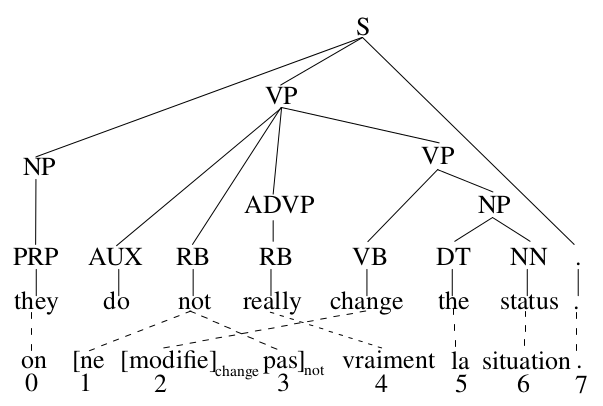
\includegraphics[scale=0.4]{crossing.png}
\caption{An example of a crossing according to \cite{fox2002phrasal}. Further explain.}\label{fig:fox}
\end{figure}

Her results are supported by others. \cite{galley2004s} focussed on the second question posed on the beginning of this Section. They generated constituency trees on the English side of the aforementioned Hansard corpus and tested how powerful a synchronous grammar should be to be consistent with the translation corpus. The power of the grammar was expressed in terms of the depth of the subtrees it generated, a standard CFG rule, that generates only single non-terminals, thus has depth 1. If rules of larger depth than 1 are needed, the non-terminal nodes of the syntactic source tree cannot be mapped bijectively to any target tree in a way consistent with the word-alignments. He found that only 19.4\% of the trees in the corpus could be entirely covered by one-depth-rules, and 85\% of the nodes (for the S alignments). Furthermore, he found that to cover the entire corpus with a grammar consistent with the allowed number of rule expansions should be no less than 17 for the S-alignments, and 23 for automatic alignments. For the English-Chinese corpus he analysed (FIBS, reference??), the coverage of low-expansion rules was even lower: 16.5\% (of the trees) for rules with a single expansion, and 100\% only with a maximum of 43\% expansions per rule.

\cite{khalilov2012statistical} confirmed the inadequacy of child-reordering in work that focusses on source reordering preliminary to translation. Using LRscore \citep{birch2010lrscore} as a measure of success, they concluded that permuting the children of nodes in a constituency tree is insufficient to reach a perfect permutation of source-words in English-Dutch and English-Spanish translation data, even when deleting up to 5 layers of nodes in the parse tree is allowed.\footnote{Their score for English-Spanish, however, is surprisingly high: around 94.}


\subsubsection{Dependency Gramars}

Not very much literature focusses on the consistency of dependency grammars with translation data, but some articles can be found on the matter. In her study about crossings, \citeauthor{fox2002phrasal} also devoted a section on dependency grammars. She observed that dependency parses are more cohesive than constituency grammars, with
2.714 crossings per sentence, compared to 2.854 for constituency grammars. A study that exclusively focusses on dependency parses was presented in \cite{hwa2002evaluating}. She investigated how well predicate argument structures agree between English and Chinese, addressing the validity of the Direct Correspondence Assumption.\footnote{Which expresses the intuition that there exists a mapping between the syntactic relationships in two sentences that are each others translation, and is thus directly allied to compositional translation} \citeauthor{hwa2002evaluating} evaluated the quality of Chinese dependency parses that were projected directly from English to Chinese through a manual word-alignment. The resulting parses ha a very low F-score (38.1), which is not surprising, as phrasal translations (multiple aligned words on source or target side) and unaligned target words always result in errors. \citeauthor{hwa2002evaluating} also observed this fact. They developed a small set of linguistically motivated rules, which boosted the F-score to 68.3, which is significantly higher, but still rather low. Also, it makes their work very specific, and hard to extend to other language pairs or contexts.

Another work along the same lines was presented by \cite{fung2006automatic}. \citeauthor{fung2006automatic} did not directly use dependency grammars, but learned cross-linguistic (English-Chinese) semantic verb frames. The learned argument mappings  had an accuracy of 89.3\%. It is unclear how their results compare to \citepos{hwa2002evaluating} results and dependency grammars in general, a fortiori because the exact nature of the learned semantic frames stays unclear.

\subsection{Formal Trees}

A second line of empirical research does not restrict source (or target) side trees to linguistic trees, but investigates the coverage of formal SCFG's. The majority of the empirical results on SCFG's focus on the coverage of binary trees \citep[e.g.,]{zhang2006synchronous,huang2009binarization}, or SCFG's in normal form \citep[e.g.,][]{sogaard2009empirical1,sogaard2009empirical2,sogaard2010can}. All concluded that the range of reordering phenomena occurring in real translation data are by far not as complicated as the worst case scenario sketched in \cite{satta2005some}.
%But also that...?

\cite{wellington2006empirical} seem to be the only one who compared their results with linguistically restricted parse trees. On several dataset (covering translation from Chinese, Romanian, Hindi, Spanish and French to English), he found that maximally 5\% of the alignments could not be explained by a completely binary tree, while the failure rate for binary trees that were constrained by monolingual parse trees on the English side climbed to 15\% for French/English to 61\% for Chinese/English. The failure rate they found for non constrained binary trees is much lower than the one found by \cite{simaan2013hats}, who reported a coverage of 71.46\% for the manual alignments of the Hansard corpus for trees with a maximal branching factor of 2. The coverage of binary trees for automatic alignments was even lower: 52.84\%. This difference between the results of \cite{wellington2006empirical} and \cite{simaan2013hats} is most likely due to a different treatment of alignment links: the latter authors used all alignment links in the dataset, while the former treated many-to-one alignment links disjunctively, focussing on lower bounds. \cite{simaan2013hats} also reported the coverage of non binarisable (permutation) trees, which is surprisingly enough not much higher: 72.14\% and 56.56\% for manual and automatic alignments, respectively.

\section{Conclusion}

In this chapter, we have discussed monolingual and bilingual compositionality, combining them blabla. The usability of monolingual syntax not yet well enough investigated .... 

\bibliography{thesisDH}
\end{document}